\documentclass[12pt]{report} % 12 pt front size
\usepackage[a4 paper, top=25mm, bottom=25mm]{geometry} % page dimensions
\headheight= 15pt
\usepackage[utf8]{inputenc} %font used is Times new roman which is the standard font for articles

%Bibliography package
\usepackage[backend=biber,style=nature]{biblatex}
% .bib is the name of the file which contains the list of references for citation
\addbibresource{references.bib}
\usepackage{fancyhdr} %for header and footer
\pagestyle{fancy}
\fancyhf{}
\usepackage{float}
\usepackage{subcaption}
\usepackage{color}
\usepackage{setspace}
\setstretch{1.5} %linespacing can be changed as per requirement
\usepackage{import}
\usepackage{titlesec}
\usepackage[export]{adjustbox}
\usepackage{tocloft}
\usepackage{supertabular}
\renewcommand\cftchapaftersnum{.}
\renewcommand\cftsecaftersnum{.}
\renewcommand\thechapter{\Roman{chapter}}
\renewcommand\thesection{\arabic{section}}
\setcounter{secnumdepth}{3} %shows detailed contents with higher sub divisions (3)
\setcounter{tocdepth}{3}
\usepackage{amsmath}
\usepackage{graphicx} %allows the user to use the graphics env
\graphicspath{{./Images/}} % The folder where the images will be uploaded
\usepackage{caption} %Allows the user to use the caption in tables and figures
\usepackage[labelfont=bf]{caption}
\captionsetup[figure]{labelsep=space,singlelinecheck=off} % The captions won`t be affected with change in line spacing and alignment of the entire document 
\usepackage[normalem]{ulem}
\useunder{\uline}{\ul}{}
\tolerance=1
\emergencystretch=\maxdimen
\hyphenpenalty=10000
\hbadness=10000
\fancyhead[R]{20th Nov. 2023}
\fancyhead[L]{Department of Mechanical Engineering, UCL}
\fancyfoot[R]{\thepage}
\renewcommand{\headrulewidth}{2pt} % the horizontal line at the top of the page
\renewcommand{\footrulewidth}{1pt} % the horizontal line at the bottom of the page

% ==================== Start of Cover Page ==================== %
\begin{document}
\begin{titlepage}
\begin{center}
        \begin{center}
        
\includegraphics[width=.70\textwidth]{Image/ucl_logo.png}
        \vspace{0.5cm}
        \end{center}
        \vspace*{0.1cm}
        % Title
        \vspace{2cm}
        {\LARGE\textbf{MECH0064 MSc Group Design Project\\}}

        % Sub-Title
        \vspace{2cm}
        {\Huge\textbf{Compact Continuum Robotic\\}}
        \vspace{0.25cm}
        {\Huge\textbf{Manipulator Platform\\}}

        \vfill

        \begin{flushleft}
        \textbf{\emph{Group members:}} \\
        Zehao Ye (23119333)~~ Zehao Ye (23119333)\\ 
        Zehao Ye (23119333)~~ Zehao Ye (23119333)\\ 
        Zehao Ye (23119333)~~ Zehao Ye (23119333)\\ 
        \textbf{\emph{Supervised by} Dr Reza Haqshenas}
        \end{flushleft}
        \vspace{0.8cm}
\end{center}
\end{titlepage}
% ==================== End of Cover Page ==================== %

%%%%% Abstract %%%%%
\section*{Abstract} 
This is the Abstract of the final report. \\
AAAAA


\vfill


\textbf{\emph{Key Words: Continuum Robotic e.g.}}
\vspace{0.8cm}
\pagenumbering{gobble}
\setcounter{page}{1}
\newpage

% =========== Start of Content page ============= %
\tableofcontents
\addtocontents{toc}{~\hfill\textbf{Page}\par}
\newpage 
% ============ End of Content page ============== %


% =========== Start of Figure List ============= %
\listoffigures
\addcontentsline{toc}{chapter}{List of Figures}
\newpage
% ============ End of Figure List ============== %



% =========== Start of Table List ============= %
\listoftables 
\addcontentsline{toc}{chapter}{List of Tables} 
\newpage
% ============ End of Table List ============== %



%%%%% Section of Question 1 %%%%%
\section{Question 1. Diode bridge circuit (4\%)} 
%%%%% Subsection of Q1 a) %%%%%
\subsection{The circuit diagram from PSCAD} 
The screen capture of the circuit diagram from PSCAD is shown in Figure \ref{fig:Q1circuitdiagram}. 
\begin{figure}[H] %[H] "corresponds to start the figure Here" 
    \centering %alignment can be flushleft or flushright
    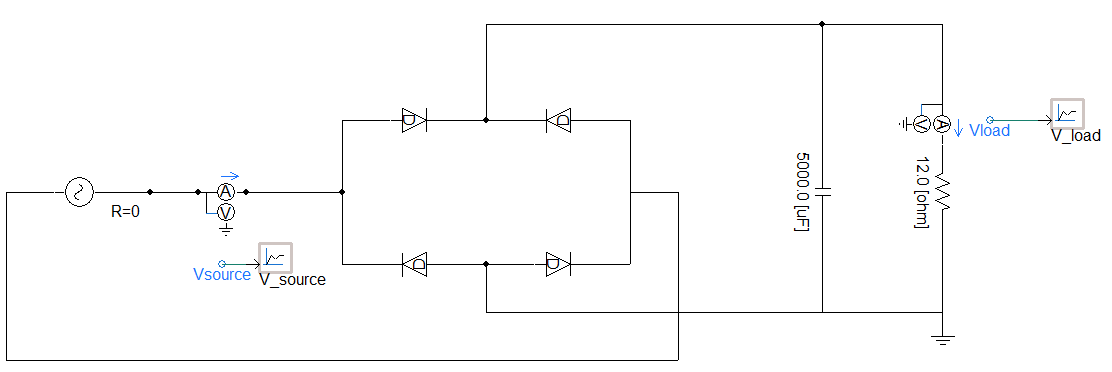
\includegraphics[width=0.9\textwidth]{Image/Q1/Q1_circuit.PNG} 
    \caption[The screen capture of your circuit diagram from PSCAD]
    {\centering \textit{\textbf{The circuit diagram:}} Screen capture about Question 1-a in PSCAD}
    \label{fig:Q1circuitdiagram}
\end{figure} %ends the image environment
%%%%% Subsection of Q1 b) %%%%%
\subsection{The instantaneous voltage measurement (5mF)} 
The screen capture of the circuit diagram from PSCAD is shown in Figure \ref{fig:Q1A2Figure}. 
\begin{figure}[H] %[H] "corresponds to start the figure Here" 
    \centering % subfigure1
    \begin{subfigure}[b]{\textwidth}
        \centering
        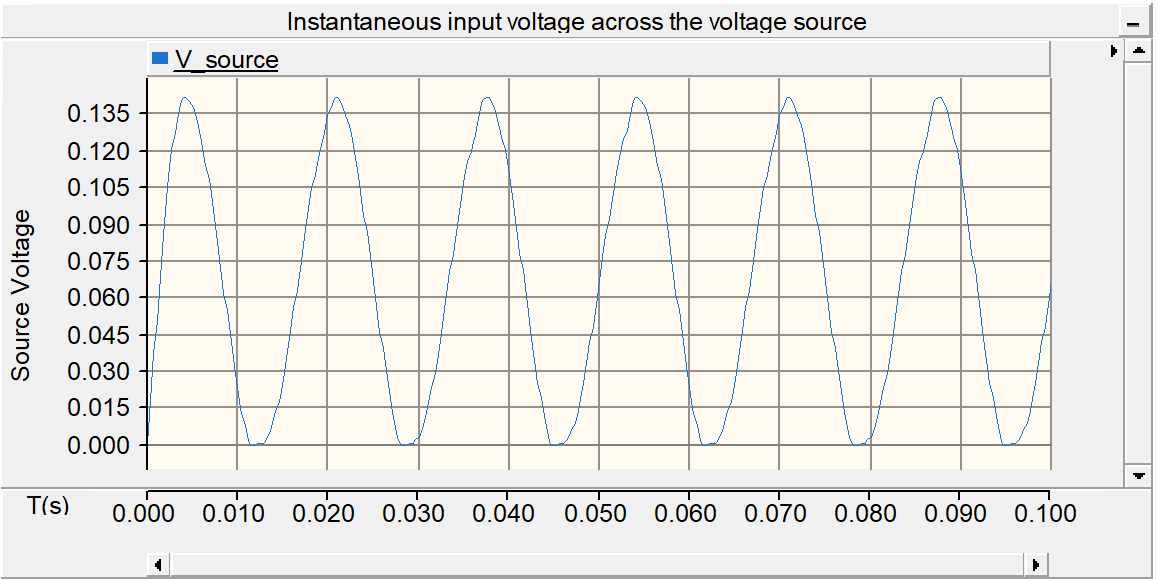
\includegraphics[width=0.7\textwidth]{Image/Q1/Q1_a2_Vsource.PNG}
        \caption{The instantaneous input voltage across the voltage source (unit: kV)}
        \label{fig:Q1A2sub1}
    \end{subfigure}
    \hfill
    \centering % subfigure2
    \begin{subfigure}[b]{\textwidth}
        \centering
        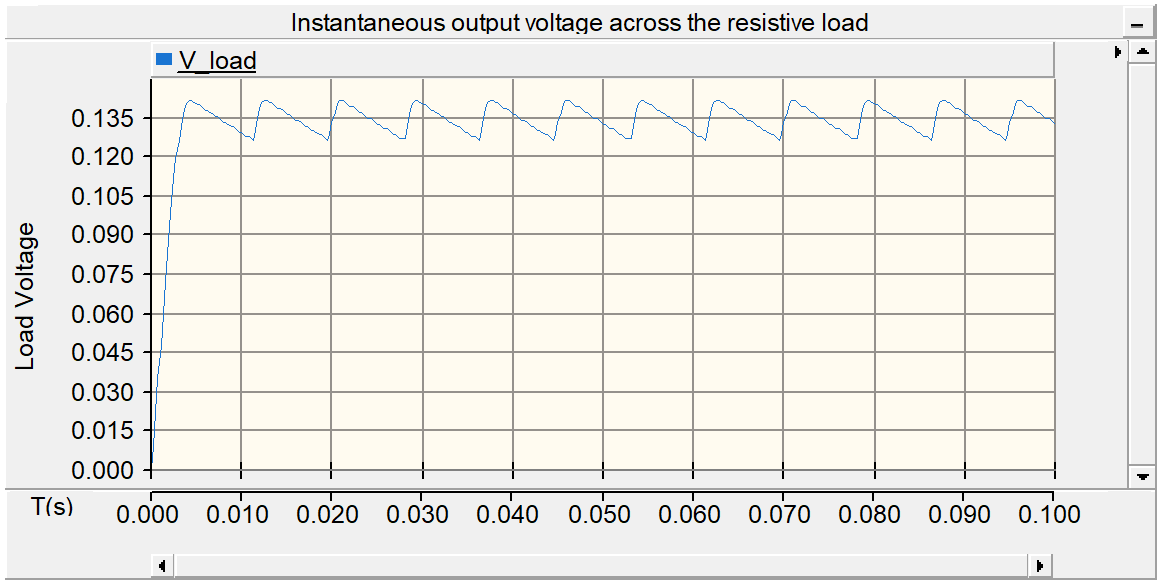
\includegraphics[width=0.7\textwidth]{Image/Q1/Q1_a2_Vload.PNG}
        \caption{The instantaneous output voltage across the resistive load (unit: kV)}
        \label{fig:Q1A2sub2}
    \end{subfigure} 
    \caption[The measured instantaneous voltages with 5mF capacitor]
    {\centering \textit{\textbf{The measured instantaneous voltages:}} V\textsubscript{source} and R\textsubscript{load}}
    \label{fig:Q1A2Figure}
\end{figure}
%%%%% Subsection of Q1 c) %%%%%
\subsection{The instantaneous voltage measurement (25mF)} 
%%%%% FIGURE %%%%%
\begin{figure}[H]
    \centering % subfigure1
    \begin{subfigure}[b]{\textwidth}
        \centering
        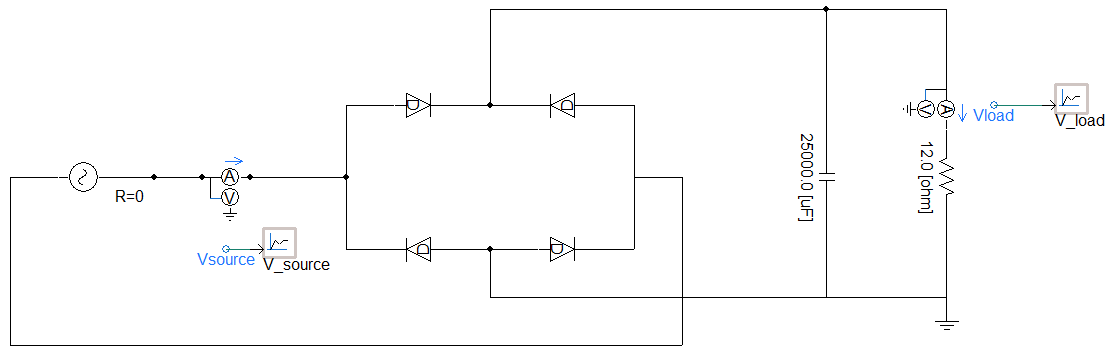
\includegraphics[width=0.9\textwidth]{Image/Q1/Q1_a3_circuit.PNG}
        \caption{The circuit diagram with different capacitor}
        \label{fig:Q1A3sub1}
    \end{subfigure}
    \hfill
    \centering % subfigure2
    \begin{subfigure}[b]{\textwidth}
        \centering
        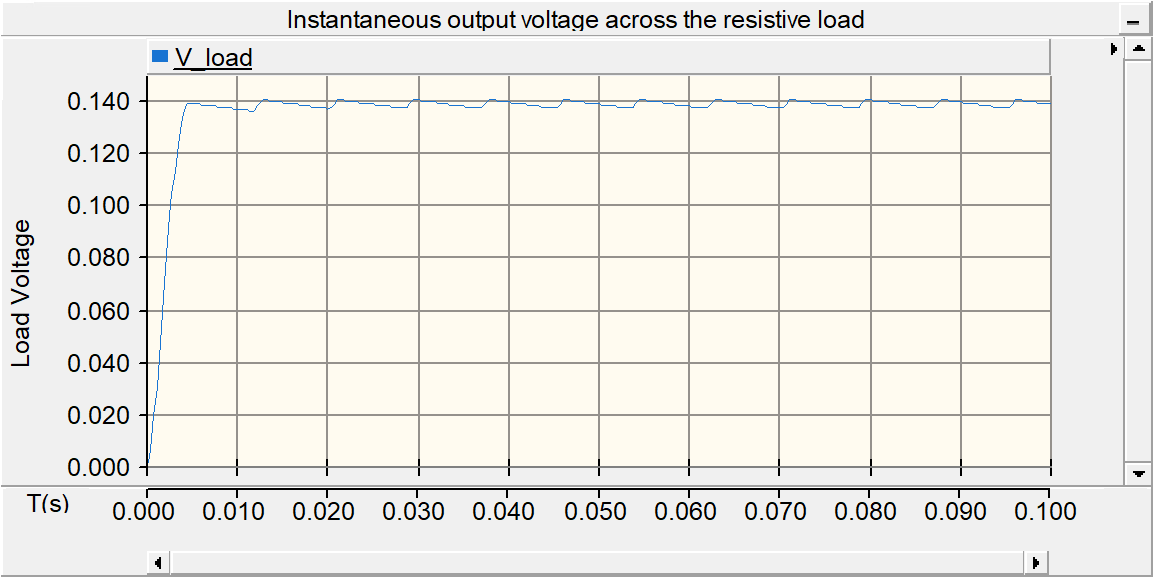
\includegraphics[width=0.7\textwidth]{Image/Q1/Q1_a3_Vload.PNG}
        \caption{The instantaneous output voltage across the resistive load (unit: kV)}
        \label{fig:Q1A3sub2}
    \end{subfigure} 
    \caption[The measured instantaneous voltages with 25mF capacitor]
    {\centering \textit{\textbf{The measured instantaneous voltages:}} R\textsubscript{load}with 25mF}
    \label{fig:Q1A3Figure}
\end{figure}
%%%%% TEXT %%%%%
To make further analysis about the impact of different capacitors on the entire circuit, the data in 
Figure \ref{fig:Q1A2sub1}, \ref{fig:Q1A2sub2}, and \ref{fig:Q1A3sub2} are exported to MATLAB. 
The peaks of the measured instantaneous voltage are labeled and the average values are plotted in Figure \ref{fig:Q1MATLAB}.
The purpose of increasing the capacitance is to reduce circuit oscillations caused by the AC power source and reduce steady state error. 
It can be observed in Figure \ref{fig:Q1MATLAB} that with a larger capacitor, the instantaneous voltage fluctuations across 
the resistive load are smaller, leading to a comparatively more stable condition.
%%%%% FIGURE %%%%%
\begin{figure}[H]
    \centering % subfigure1
    \begin{subfigure}[b]{\textwidth}
        \centering
        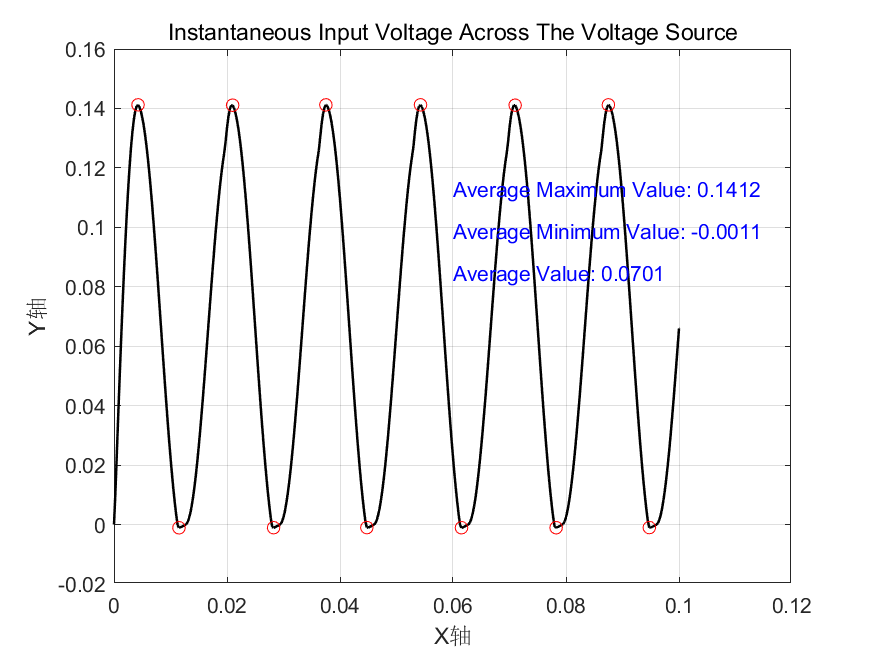
\includegraphics[width=0.65\textwidth]{Image/Q1/Q1A2Vsource.png}
        \caption{The instantaneous input voltage across the voltage source in MATLAB}
        \label{fig:Q1MATLABsub1}
    \end{subfigure}
    \hfill
    \centering % subfigure2
    \begin{subfigure}[b]{\textwidth}
        \centering
        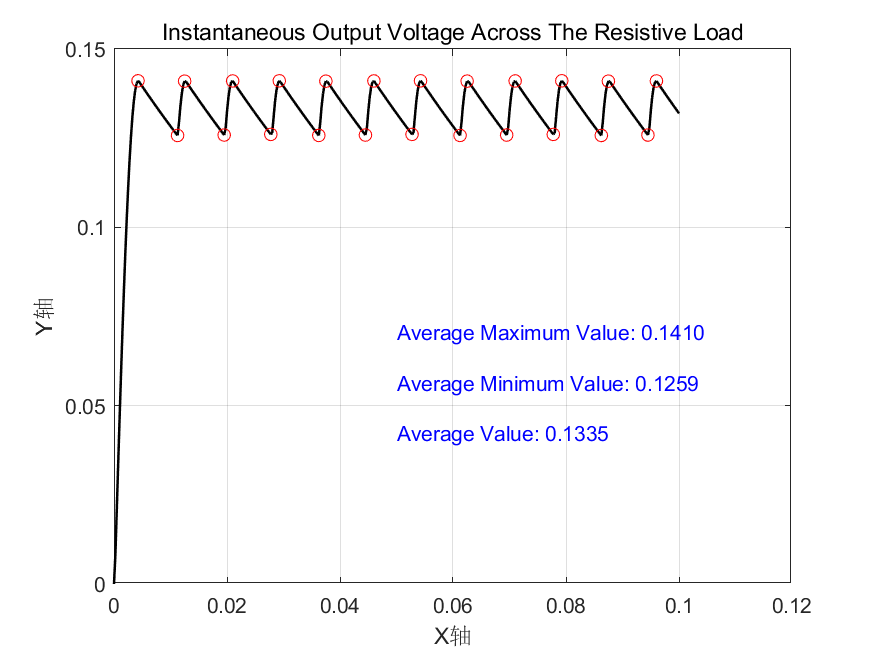
\includegraphics[width=0.65\textwidth]{Image/Q1/Q1A2Vload.png}
        \caption{The instantaneous output voltage across the resistive load (5mF) in MATLAB}
        \label{fig:Q1MATLABsub2}
    \end{subfigure} 
    \hfill
    \centering % subfigure3
    \begin{subfigure}[b]{\textwidth}
        \centering
        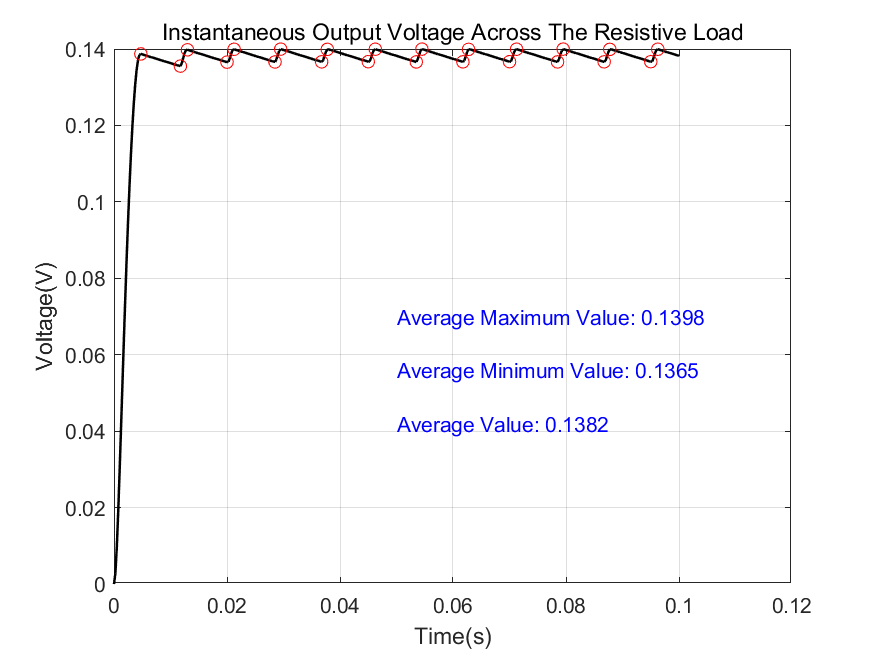
\includegraphics[width=0.65\textwidth]{Image/Q1/Q1A3Vload.png}
        \caption{The instantaneous output voltage across the resistive load (25mF) in MATLAB}
        \label{fig:Q1MATLABsub3}
    \end{subfigure} 
    \caption[The processed instantaneous voltage measurements in MATLAB]
    {\centering \textit{\textbf{The processed instantaneous voltages:}} Processed in MATLAB, the unit in the MATLAB plots are kiloVolt(kV)}
    \label{fig:Q1MATLAB}
\end{figure}
\newpage
%%%%%%%%%%%%%%%%%%%%%%%%%%%%%%%%%%%% NEW SECTION %%%%%%%%%%%%%%%%%%%%%%%%%%%%%%%%%%%%%%%%


%%%%% Section of Question 2 %%%%%
\section{Question 2. Equivalent transformer (4\%)} 
%%%%% Subsection of Q2 a) %%%%%
\subsection{The circuit diagram from PSCAD}
The screen capture of the circuit diagram from PSCAD about the resistive, inductive, and capacitive laod 
are shown in Figure \ref{fig:Q2circuit_sub1}, \ref{fig:Q2circuit_sub2}, and \ref{fig:Q2circuit_sub3} respectively. 
%%%%% FIGURE %%%%%
\begin{figure}[H]
    \centering % subfigure1
    \begin{subfigure}[b]{\textwidth}
        \centering
        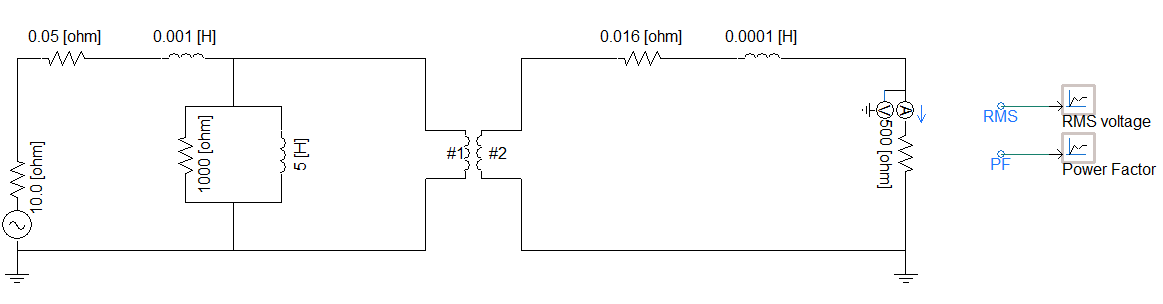
\includegraphics[width=0.9\textwidth]{Image/Q2/Q2_resistor_circuit.PNG}
        \caption{The circuit diagram with the resistive load}
        \label{fig:Q2circuit_sub1}
    \end{subfigure}
    \hfill
    \centering % subfigure2
    \begin{subfigure}[b]{\textwidth}
        \centering
        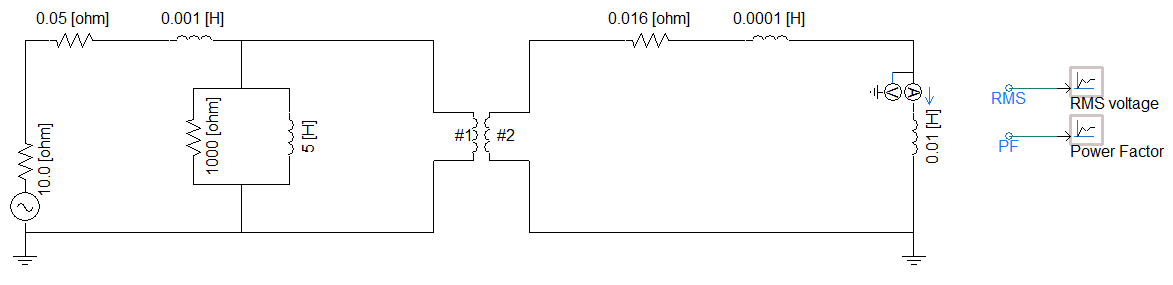
\includegraphics[width=0.9\textwidth]{Image/Q2/Q2_inductor_circuit.PNG}
        \caption{The circuit diagram with the inductive load}
        \label{fig:Q2circuit_sub2}
    \end{subfigure} 
    \hfill
    \centering % subfigure3
    \begin{subfigure}[b]{\textwidth}
        \centering
        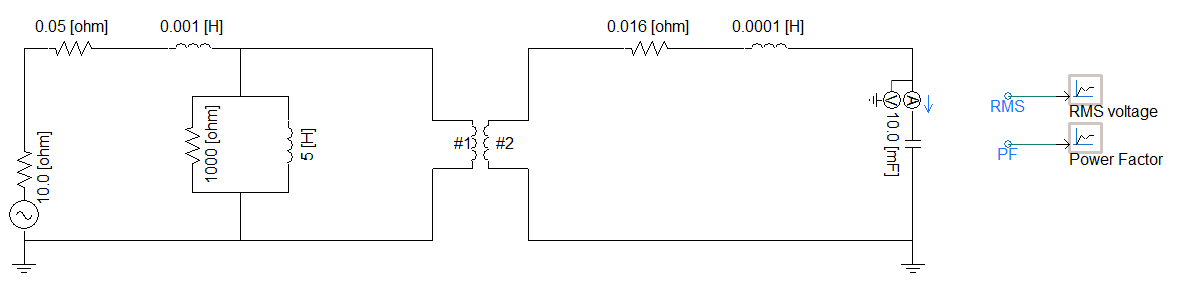
\includegraphics[width=0.9\textwidth]{Image/Q2/Q2_capacitor_circuit.PNG}
        \caption{The circuit diagram with the capacitive load}
        \label{fig:Q2circuit_sub3}
    \end{subfigure} 
    \caption[The circuit diagrams of the different loads]
    {\centering \textit{\textbf{The circuit diagrams:}} resistive, inductive, and capacitive load}
    \label{fig:Q2circuitdiagram}
\end{figure}
\newpage
%%%%% Subsection of Q2 b) %%%%%
\subsection{The measurement across the resistive load}
The RMS voltage (analogue) and power factor (angular) about the resistive laod are shown in Figure \ref{fig:Q2R_RMS} and \ref{fig:Q2R_PF}. 
%%%%% FIGURE %%%%%
\begin{figure}[H]
    \centering % subfigure1
    \begin{subfigure}[b]{\textwidth}
        \centering
        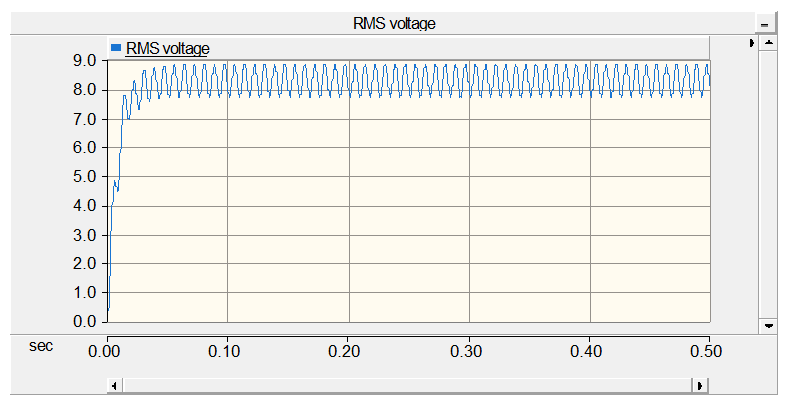
\includegraphics[width=0.9\textwidth]{Image/Q2/Q2_resistor_RMS.PNG}
        \caption{The RMS voltage about the resistive load (unit: kV)}
        \label{fig:Q2R_RMS}
    \end{subfigure}
    \hfill
    \centering % subfigure2
    \begin{subfigure}[b]{\textwidth}
        \centering
        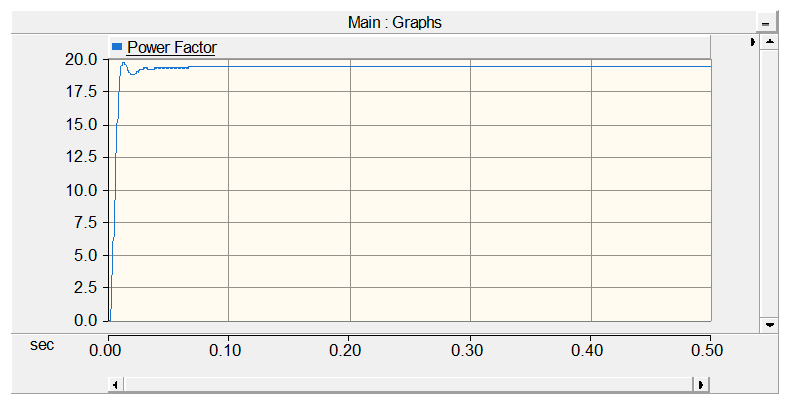
\includegraphics[width=0.9\textwidth]{Image/Q2/Q2_resistor_PF.PNG}
        \caption{The power factor about the resistive load (unit: degree~$^\circ$)}
        \label{fig:Q2R_PF}
    \end{subfigure} 
    \caption[The RMS voltage and power factor about the resistive load ]
    {\centering \textit{\textbf{The measurements about the resistive load:}} RMS Voltage(analogue) and Power Factor(angular)}
    \label{fig:Q2R}
\end{figure}
\newpage
%%%%% Subsection of Q2 c) %%%%%
\subsection{The measurement across the inductive load}
The RMS voltage (analogue) and power factor (angular) about the inductive laod are shown in Figure \ref{fig:Q2L_RMS} and \ref{fig:Q2L_PF}. 
%%%%% FIGURE %%%%%
\begin{figure}[H]
    \centering % subfigure1
    \begin{subfigure}[b]{\textwidth}
        \centering
        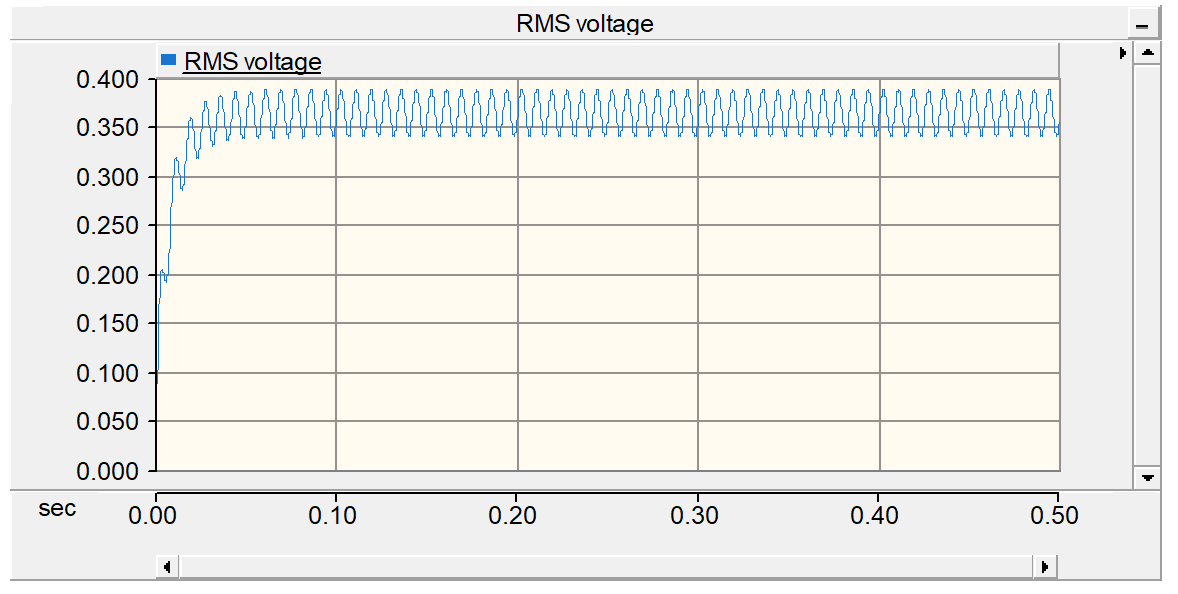
\includegraphics[width=0.9\textwidth]{Image/Q2/Q2_inductor_RMS.PNG}
        \caption{The RMS voltage about the inductive load (unit: kV)}
        \label{fig:Q2L_RMS}
    \end{subfigure}
    \hfill
    \centering % subfigure2
    \begin{subfigure}[b]{\textwidth}
        \centering
        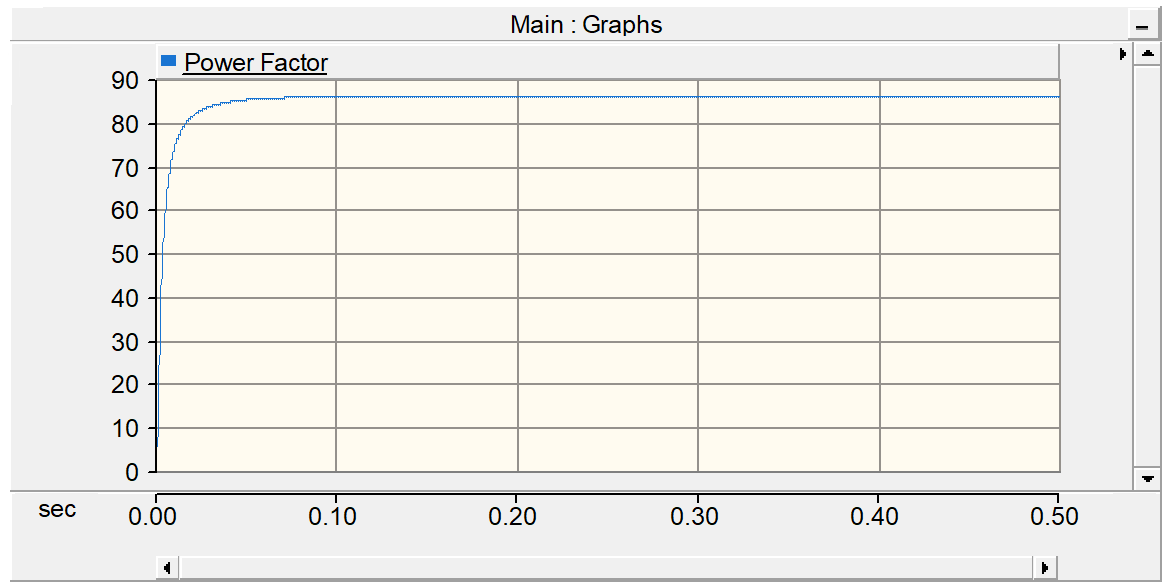
\includegraphics[width=0.9\textwidth]{Image/Q2/Q2_inductor_PF.PNG}
        \caption{The power factor about the inductive load (unit: degree~$^\circ$)}
        \label{fig:Q2L_PF}
    \end{subfigure} 
    \caption[The RMS voltage and power factor about the inductive load ]
    {\centering \textit{\textbf{The measurements about the inductive load:}} RMS Voltage(analogue) and Power Factor(angular)}
    \label{fig:Q2L}
\end{figure}
\newpage
%%%%% Subsection of Q2 d) %%%%%
\subsection{The measurement across the capacitive load}
The RMS voltage (analogue) and power factor (angular) about the capacitive laod are shown in Figure \ref{fig:Q2C_RMS} and \ref{fig:Q2C_PF}. 
%%%%% FIGURE %%%%%
\begin{figure}[H]
    \centering % subfigure1
    \begin{subfigure}[b]{\textwidth}
        \centering
        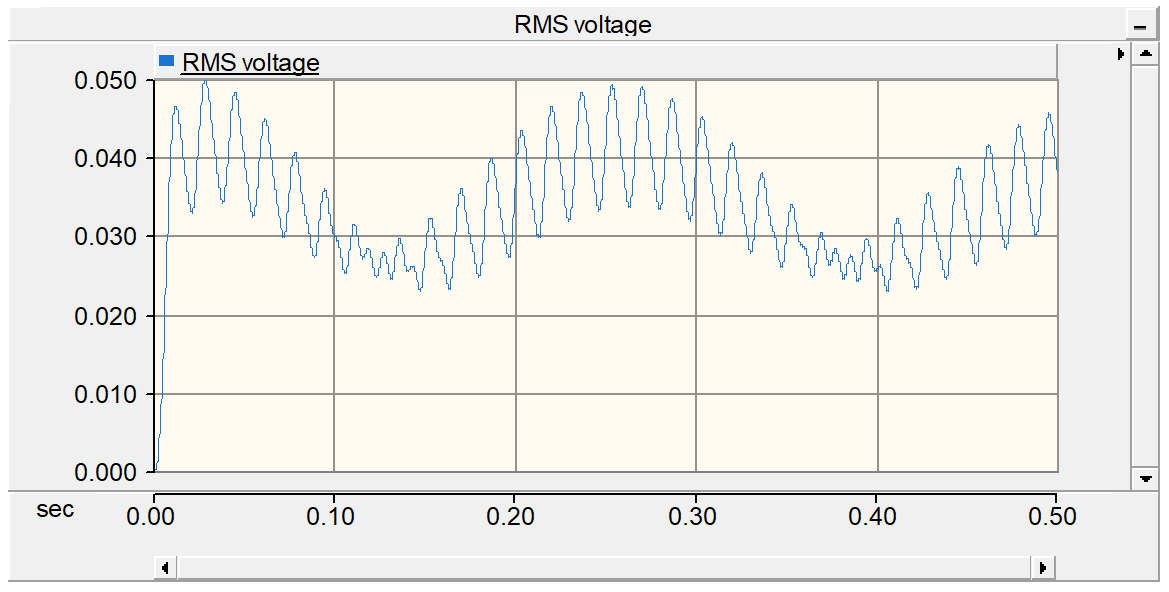
\includegraphics[width=0.9\textwidth]{Image/Q2/Q2_capacitor_RMS.PNG}
        \caption{The RMS voltage about the capacitive load (unit: kV)}
        \label{fig:Q2C_RMS}
    \end{subfigure}
    \hfill
    \centering % subfigure2
    \begin{subfigure}[b]{\textwidth}
        \centering
        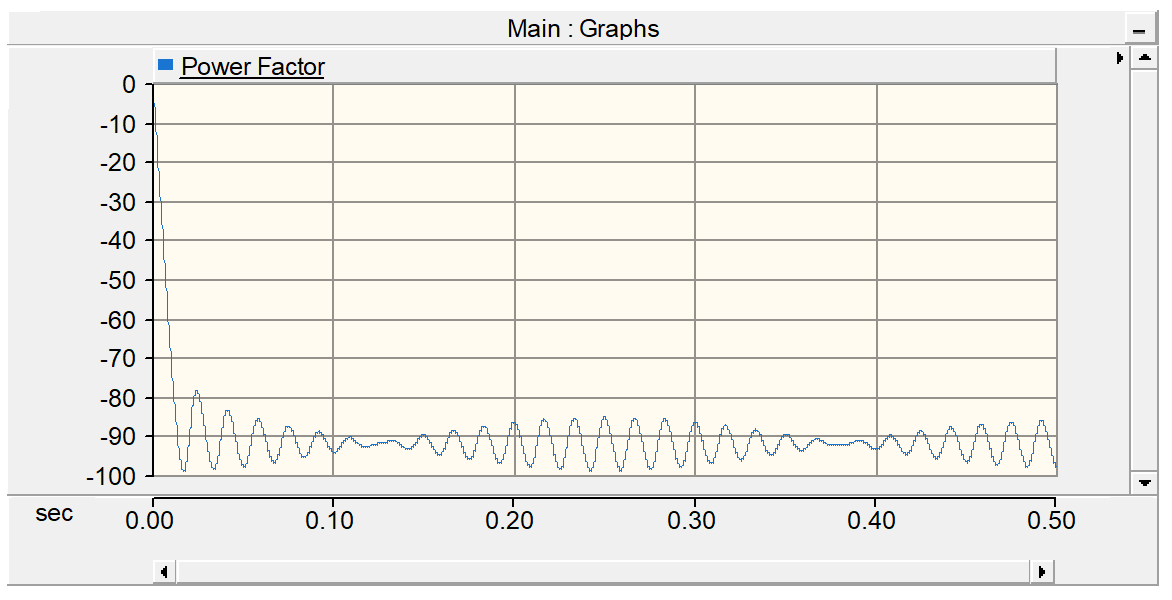
\includegraphics[width=0.9\textwidth]{Image/Q2/Q2_capacitor_PF.PNG}
        \caption{The power factor about the capacitive load (unit: degree~$^\circ$)}
        \label{fig:Q2C_PF}
    \end{subfigure} 
    \caption[The RMS voltage and power factor about the capacitive load ]
    {\centering \textit{\textbf{The measurements about the capacitive load:}} RMS Voltage(analogue) and Power Factor(angular)}
    \label{fig:Q2C}
\end{figure}
\newpage
%%%%%%%%%%%%%%%%%%%%%%%%%%%%%%%%%%%% NEW SECTION %%%%%%%%%%%%%%%%%%%%%%%%%%%%%%%%%%%%%%%%



%%%%% Section of Question 3 %%%%%
\section{Question 3. Faulted 3-$\Phi$ network PART 1 (4\%)} 
\newpage
%%%%%%%%%%%%%%%%%%%%%%%%%%%%%%%%%%%% NEW SECTION %%%%%%%%%%%%%%%%%%%%%%%%%%%%%%%%%%%%%%%%



%%%%% Section of Question 4 %%%%%
\section{Question 4. Faulted 3-$\Phi$ network PART 2 (5\%)} 
\newpage
%%%%%%%%%%%%%%%%%%%%%%%%%%%%%%%%%%%% NEW SECTION %%%%%%%%%%%%%%%%%%%%%%%%%%%%%%%%%%%%%%%%



%%%%% Section of Question 5 %%%%%
\section{Question 5. Faulted 3-$\Phi$ network PART 3 (8\%)} 
\newpage
%%%%%%%%%%%%%%%%%%%%%%%%%%%%%%%%%%%% NEW SECTION %%%%%%%%%%%%%%%%%%%%%%%%%%%%%%%%%%%%%%%%



%%%%% Section of Question 6 %%%%%
\section{Question 6. . Faulted Network Analysis (10\%)} 
\newpage
%%%%%%%%%%%%%%%%%%%%%%%%%%%%%%%%%%%% NEW SECTION %%%%%%%%%%%%%%%%%%%%%%%%%%%%%%%%%%%%%%%%

\printbibliography[title = {References}]
\addcontentsline{toc}{chapter}{References}
\end{document}
%------------------------------------------The Document Ends here--------------------------------------------